\chapter[Materiais e Métodos]{Materiais e Métodos}

A metodologia será através de pesquisa e escolha dos componentes que serão utilizados para desenvolvimento do sistema. Neste trabalho nos atentaremos a desenvolver o sistema embarcado capaz de realizar as operações necessárias para cumprir os objetivos descritos na sessão \ref{OBJETIVOS}.

Na busca de uma solução para o sistema proposto, desmembrou-se o diagrama (Figura \ref{fig:blocos}) a fim de modularizar o processo. Primeiramente, ao receber a imagem , deve-se definir qual o fator de redimensionamento será usado. O que definirá esse fator pode ser dado por uma métrica (cálculos realizados sobre a imagem) ou uma regra (enviar uma imagem com tamanho original e a próxima com um quarto desse tamanho), previamente definida, baseada nas características da imagem em geral. Para realizar o redimensionamento, com o fator já definido, é necessário aplicar o algoritmo baseado na DCT, semelhante ao apresentado na sessão 2.2. Para a codificação, serão utilizados \textit{codecs} já disponíveis para a codificação (em JPEG e H.264). A decodificação segue o mesmo princípio. Por fim, a reconstrução desfaz o processo de redimensionamento anterior

\begin{figure}[h]
	\centering
	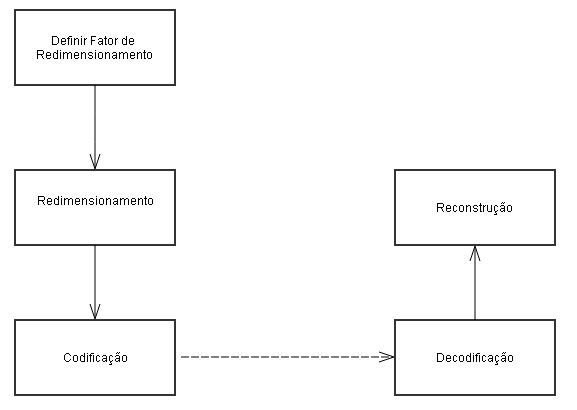
\includegraphics[scale=.8]{figuras/BLOCOS.png}
	\caption{Diagrama de blocos proposto para solução.}
	\label{fig:blocos}
\end{figure}

Assim, para escolher o kit de desenvolvimento que seria utilizado, após pesquisa
de diferentes modelos e fabricantes, o primeiro passo foi escolher entre dois grupos distintos
: DSP (do inglês, \textit{digital signal processor}) e FPGAs (do inglês,\textit{ Field Programmable Gate
Arrays}).

FPGAs são circuitos integrados digitais que possuem um conjunto de blocos lógicos
organizados em forma de matriz e respectivas interligações, que podem ser configuradas
de modo a criar um circuito digital que se pretenda implementar \cite{meixedo2008metodologias}.

Já os DSP são, como o nome diz, processadores dedicados ao processamento de sinas digitais. Propriedades interessantes desse processadores são:
\begin{itemize}
	\item[•] Apresentam um consumo muito menor quando comparado, por exemplo, com um
processador \textit{Pentium}.
	\item[•] Estão otimizados para a repetição de operações (\textit{looping}) comuns nos algoritmos de
processamento de sinal, ou seja, multiplicar e adicionar (\textit{Multiply and Accumutate} -
MAC);
\item[•] Possuem periféricos próprios que permitem uma interface de entrada/saída eficiente
com outros dispositivos, como por exemplo, microfone e alto-falante. 
\end{itemize}

Para a escolha do \textit{kit}, os seguintes aspectos foram priorizados: velocidade de processamento(\textit{clock}),
facilidade de uso, quantidade de referências existentes e disponibilidade
de ferramentas específicas para codificação de imagens (bibliotecas prontas), prazo de
aquisição do equipamento, consumo energético e preço.

Devido a facilidade de uso (experiência prévia do desenvolver), disponibilidade de bibliotecas específicas para processamento de imagens (\textit{codecs} H.264 e JPEG) e baixo consumo optou-se por utilizar um DSP do fabricante \textit{Texas Instruments}. Essas características se sobresairam em frente as FPGAs mais populares das fabricantes Altera e Xilinx.

O \textit{kit} escolhido foi o TMS320C5515 eZdsp (figura 12 ), fabricado pela \textit{Texas Instruments},dentre suas características temos:

\begin{itemize}
	\item[•] Realiza de 200 a 240 milhões de MACs  por segundo;
	\item[•] \textit{Clock}: 60, 75, 100 e 120 MHz;
	\item[•] Suporte para DSP / BIOS ™ do kernel em tempo real;
	\item[•] 512-kB \textit{SPI Flash} e 1-MB \textit{SDRAM}. 
\end{itemize}

\newpage

\begin{figure}[h]
	\centering
	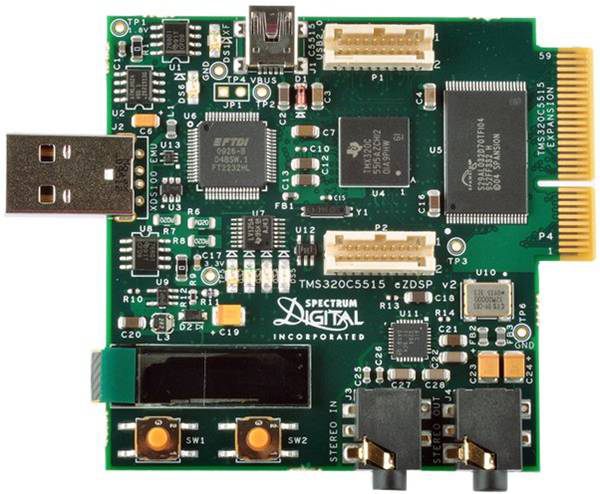
\includegraphics[scale=0.45]{figuras/DSP.jpg}
	\caption{\textit{Kit} de desenvolvimento TMS320C5515 eZdsp(\textit{Texas Instrument}).}
	\label{dsp}
\end{figure}